\documentclass[a4paper]{article}

\usepackage[a4paper, total={18cm, 26cm}]{geometry}
\usepackage[T1]{fontenc} % needed by beramono
\usepackage{textcomp}
% beramono.sty and MnSymbol.sty come with texlive-fonts-extra in Debian
\usepackage[scaled=0.85]{beramono} % tt font supporting slshape and zero with dot
\usepackage{MnSymbol} % fancy symbols for line-breaks
\usepackage[utf8]{inputenc}
\usepackage{listingsutf8}  % code listings, comes with texlive-latex-recommended
%\usepackage{listings}
\usepackage{xcolor}
\usepackage{verbatim}
\usepackage{graphicx} % \includegraphics[width=\textwidth]{image.png}
\usepackage{float}
\usepackage{hyperref}

\protected\def\plusminus{\ensuremath{\pm}}
\DeclareUnicodeCharacter{C2B1}{\plusminus}
\DeclareUnicodeCharacter{001B}{}

\lstset{
  inputencoding=utf8,
  literate={±}{\plusminus}1
}

\lstdefinestyle{bwC++}{
  language=C++,morekeywords={concept,consteval,constinit,constexpr,co_await,co_return,co_yield,requires},
  basicstyle=\ttfamily,
  keywordstyle=\bfseries,
  stringstyle=\slshape,
  commentstyle=\slshape,
  morecomment=[s][\bfseries\slshape]{/**}{*/},
  tabsize=4,
  showstringspaces=false,
  breaklines=true, breakatwhitespace=true,
  prebreak={\hbox{\quad$\rhookswarrow$}},
  postbreak={\hbox{$\lhookrightarrow$}},
  breakindent={-8pt}, breakautoindent=false,
  numbers=left, numberstyle=\tiny,
  frameshape={RYR}{N}{N}{YYY} %frame=tb,frameround=tttt
}

\lstdefinestyle{colorC++}{
  language=C++,morekeywords={concept,consteval,constinit,constexpr,co_await,co_return,co_yield,requires},
  basicstyle=\ttfamily,
  keywordstyle=\textcolor{blue},
  stringstyle=\slshape\textcolor{red!70!black},
  commentstyle=\slshape\textcolor{green!50!black},
  morecomment=[s][\bfseries\slshape\textcolor{green!50!black}]{/**}{*/},
  tabsize=4,
  showstringspaces=false,
  breaklines=true, breakatwhitespace=true,
  prebreak={\hbox{\quad\textcolor{red}{$\rhookswarrow$}}},
  postbreak={\hbox{\textcolor{red}{$\lhookrightarrow$}}},
  breakindent={-8pt}, breakautoindent=false,
  numbers=left, numberstyle=\tiny,
  frameshape={RYR}{N}{N}{YYY} %frame=tb,frameround=tttt
}

\lstdefinestyle{colorBash}{
  language=bash,
  basicstyle=\ttfamily,
  keywordstyle=\textcolor{blue},
  stringstyle=\slshape\textcolor{red!70!black},
  commentstyle=\slshape\textcolor{green!50!black},
  morecomment=[s][\bfseries\slshape\textcolor{green!50!black}]{/**}{*/},
  tabsize=4,
  showstringspaces=false,
  breaklines=true, breakatwhitespace=true,
  prebreak={\hbox{\quad\textcolor{red}{$\rhookswarrow$}}},
  postbreak={\hbox{\textcolor{red}{$\lhookrightarrow$}}},
  breakindent={-8pt}, breakautoindent=false,
  numbers=left, numberstyle=\tiny,
  frameshape={RYR}{N}{N}{YYY} %frame=tb,frameround=tttt
}

\title{sP Exam Mini-Project}
\author{Nikolaj Kofod Krogh}
\begin{document}
\pagenumbering{gobble}
\newpage
\pagenumbering{arabic}
\maketitle

\addcontentsline{toc}{section}{Conclusion}
\section*{Conclusion}
I have included CMakeLists.txt that shows how to build the project and run the tests. It is included as the first listing.
\newline
\newline
As we can see from the benchmark it is much faster to run the simulation in parallel (22.1 s) compared to running on a single thread (89.7 s), because it is possible to use multiple threads and thereby distribute the load.

\addcontentsline{toc}{section}{Figures}
\begin{figure}[H]
  \centering
  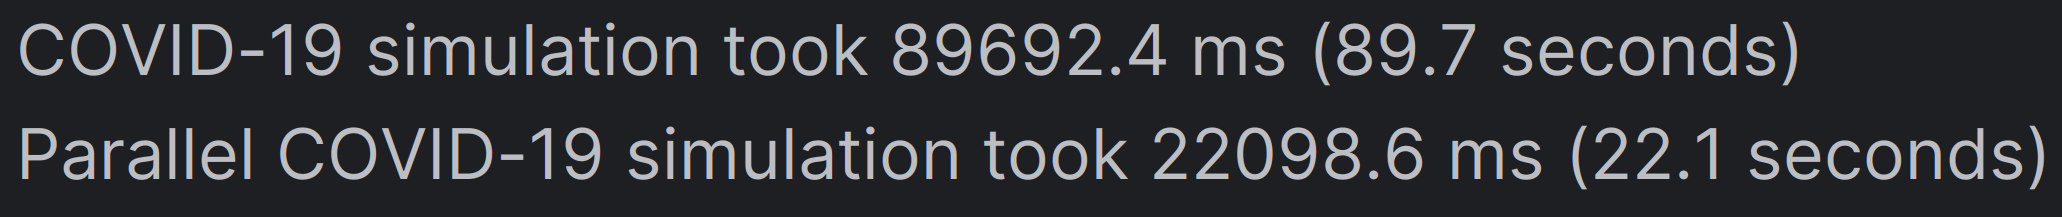
\includegraphics[width=0.7\textwidth]{images/benchmark.png}
  \caption{benchmark}
\end{figure}

\begin{figure}[H]
  \centering
  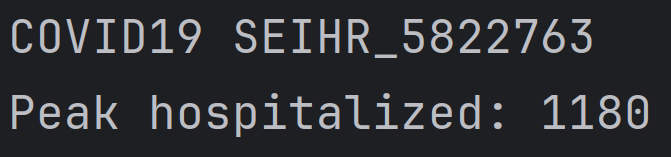
\includegraphics[width=0.7\textwidth]{images/peak_hospitalized_ndk.png}
  \caption{peak hospitalized NDK}
\end{figure}

\begin{figure}[H]
  \centering
  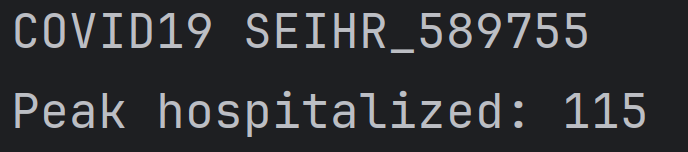
\includegraphics[width=0.7\textwidth]{images/peak_hospitalized_nnj.png}
  \caption{peak hospitalized NNJ}
\end{figure}

\begin{figure}[H]
  \centering
  
\includegraphics[width=0.7\textwidth]{images/average_peak_over_100_simulations.png}
  \caption{average peak over 100 simulations with a population size of 10000}
\end{figure}

\begin{figure}[H]
  \centering
  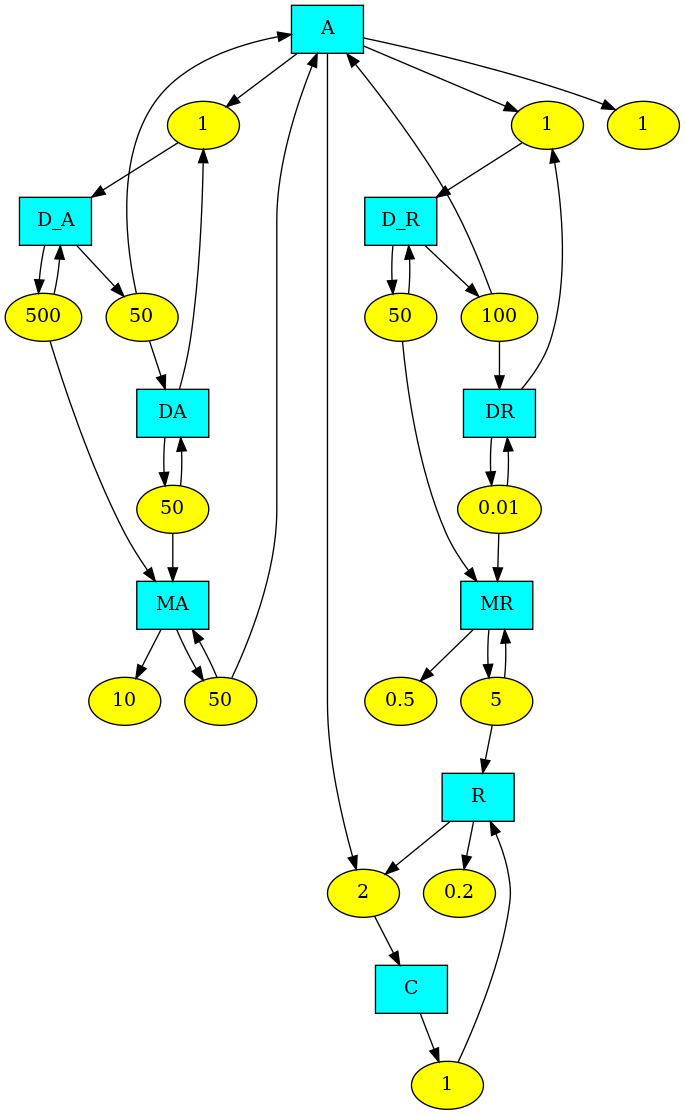
\includegraphics[width=0.7\textwidth]{images/Circadian_Rhythm_tree}
  \caption{Circadian Rhythm tree}
\end{figure}

\begin{figure}[H]
  \centering
  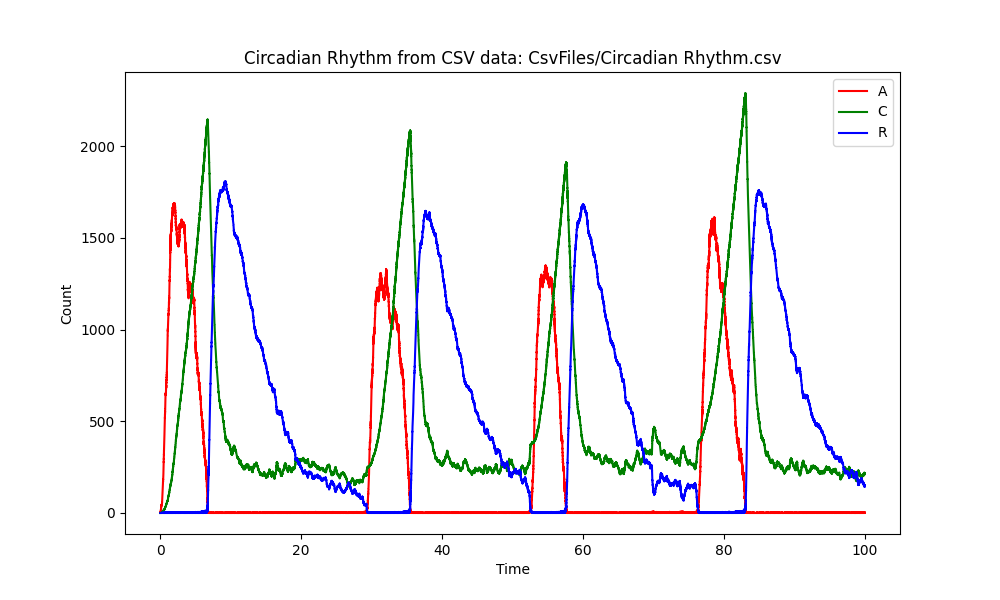
\includegraphics[width=0.7\textwidth]{images/Circadian Rhythm.png}
  \caption{Circadian Rhythm in images}
\end{figure}

\begin{figure}[H]
  \centering
  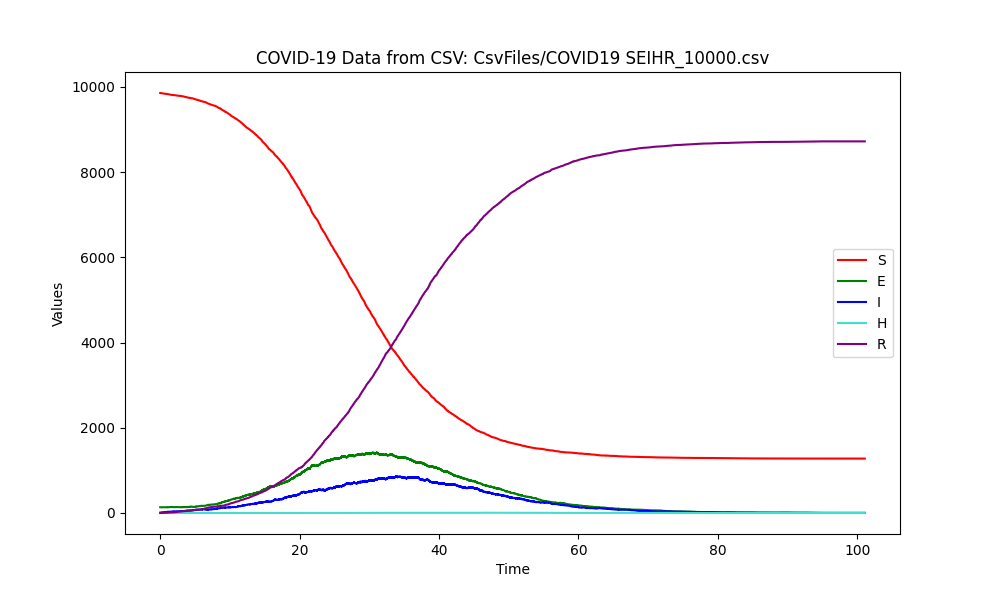
\includegraphics[width=0.7\textwidth]{images/COVID19 SEIHR_10000.png}
  \caption{COVID19 population size 10000}
\end{figure}

\begin{figure}[H]
  \centering
  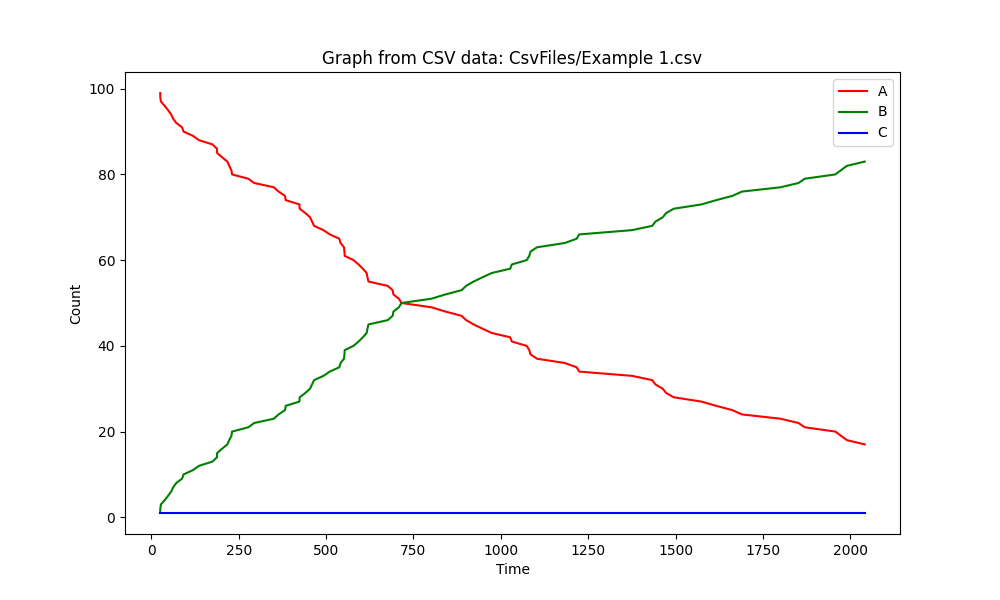
\includegraphics[width=0.7\textwidth]{images/Example 1.png}
  \caption{Example 1}
\end{figure}

\begin{figure}[H]
  \centering
  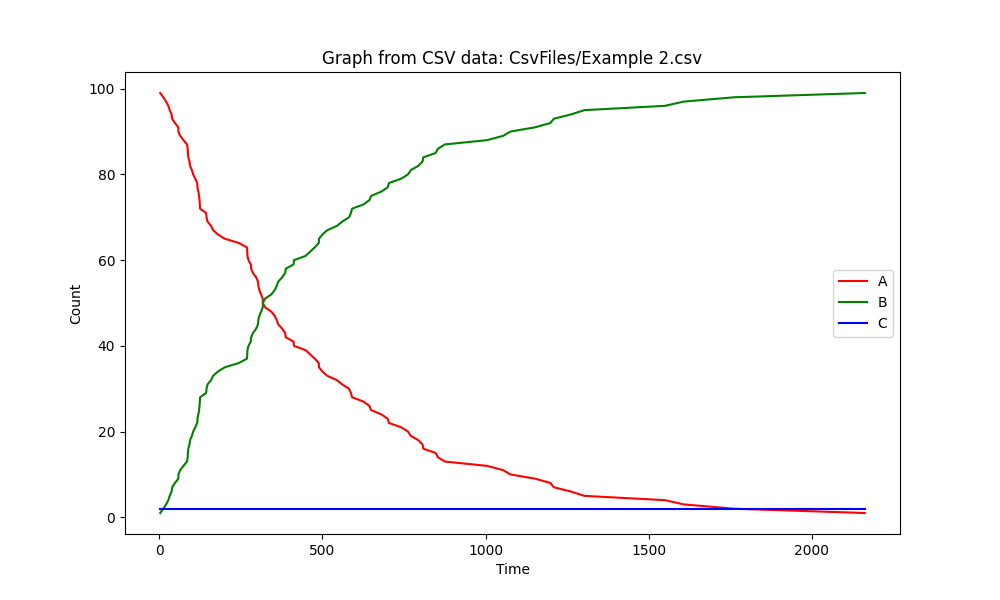
\includegraphics[width=0.7\textwidth]{images/Example 2.png}
  \caption{Example 2}
\end{figure}

\begin{figure}[H]
  \centering
  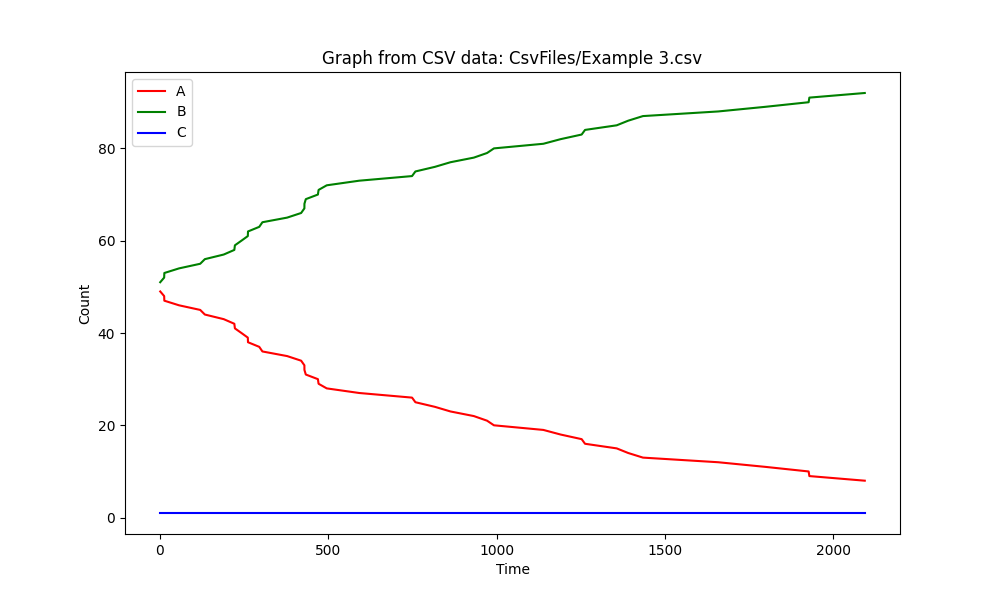
\includegraphics[width=0.7\textwidth]{images/Example 3.png}
  \caption{Example 3}
\end{figure}

\addcontentsline{toc}{section}{CMakeLists}
\lstinputlisting[style=colorBash,caption={./CMakeLists.txt}, label={lst:cmakelists}]{./CMakeLists.txt}
\addcontentsline{toc}{section}{main}
\lstinputlisting[style=colorC++,caption={./main.cpp}]{./main.cpp}
\addcontentsline{toc}{section}{Molecule}
\lstinputlisting[style=colorC++,caption={./Molecule.h}]{./Molecule.h}
\lstinputlisting[style=colorC++,caption={./Molecule.cpp}]{./Molecule.cpp}
\addcontentsline{toc}{section}{Reaction}
\lstinputlisting[style=colorC++,caption={./Reaction.h}]{./Reaction.h}
\lstinputlisting[style=colorC++,caption={./Reaction.cpp}]{./Reaction.cpp}
\addcontentsline{toc}{section}{Environment}
\lstinputlisting[style=colorC++,caption={./Environment.h}]{./Environment.h}
\lstinputlisting[style=colorC++,caption={./Environment.cpp}]{./Environment.cpp}
\addcontentsline{toc}{section}{Vessel}
\lstinputlisting[style=colorC++,caption={./Vessel.h}]{./Vessel.h}
\lstinputlisting[style=colorC++,caption={./Vessel.cpp}]{./Vessel.cpp}
\lstinputlisting[style=colorC++,caption={./Tests/VesselTests.cpp}]{./Tests/VesselTests.cpp}
\addcontentsline{toc}{section}{Arrow}
\lstinputlisting[style=colorC++,caption={./Arrow.h}]{./Arrow.h}
\lstinputlisting[style=colorC++,caption={./Arrow.cpp}]{./Arrow.cpp}
\addcontentsline{toc}{section}{Symbol Table}
\lstinputlisting[style=colorC++,caption={./SymbolTable.h}]{./SymbolTable.h}
\lstinputlisting[style=colorC++,caption={./Tests/SymbolTableTests.cpp}]{./Tests/SymbolTableTests.cpp}
\addcontentsline{toc}{section}{Simulation}
\lstinputlisting[style=colorC++,caption={./Simulation.h}]{./Simulation.h}
\addcontentsline{toc}{section}{Parallel Simulation}
\lstinputlisting[style=colorC++,caption={./ParallelSimulation.h}]{./ParallelSimulation.h}
\addcontentsline{toc}{section}{Benchmark}
\lstinputlisting[style=colorC++,caption={./benchmark.cpp}]{./benchmark.cpp}
\lstinputlisting[style=colorC++,caption={./benchmark.h}]{./benchmark.h}
\addcontentsline{toc}{section}{Graphical Simulation}
\lstinputlisting[style=colorC++,caption={./CsvFiles/graphical\_simulation.py}]{./CsvFiles/graphical_simulation.py}
\end{document}
